\documentclass[%twoside, open=right
]{scrreprt}

%\usepackage{lmodern}
\usepackage{fouriernc}
\usepackage[T1]{fontenc}


\input{Qcircuit}

\usepackage[english]{babel}
\usepackage[utf8]{inputenc}
\usepackage{amsmath, amssymb, amsxtra}
\usepackage{xspace, braket}
\usepackage{setspace}

\usepackage{sistyle} %Units
\usepackage{cleveref}
%\usepackage{hyperref}
\usepackage{cancel}
\usepackage{lipsum}
%\usepackage{slashbox}

\usepackage{graphicx}
\usepackage[justification=centering]{caption}
\usepackage{subcaption}
\usepackage{wrapfig}

\renewcommand*{\dictumauthorformat}[1]{#1}

\usepackage[nottoc, notlof, notlot]{tocbibind}

\newcommand{\defi}{\xspace\ensuremath{\overset{\text{\tiny def}}{=}}\xspace}

\newcommand{\g}{\ensuremath{\ket{0}}\xspace}
\newcommand{\e}{\ensuremath{\ket{1}}\xspace}

\newcommand{\ff}{\ensuremath{\ket{g}}\xspace}
\newcommand{\ee}{\ensuremath{\ket{e}}\xspace}
\newcommand{\rr}{\ensuremath{\ket{r}}\xspace}
\newcommand{\bg}{\ensuremath{\bra{g}}\xspace}
\newcommand{\be}{\ensuremath{\bra{e}}\xspace}
\newcommand{\br}{\ensuremath{\bra{r}}\xspace}


\newcommand{\mat}{\emph{Mathematica}\xspace}
\newcommand{\matC}[1]{\textsl{\texttt{#1}}}

\newcommand{\dd}{\ensuremath{\mathrm d}\xspace}

\newcommand{\om}{\omega}
\newcommand{\Om}{\Omega}
\newcommand{\ga}{\gamma}
\newcommand{\Ga}{\Gamma}
\newcommand{\de}{\delta}
\newcommand{\De}{\Delta}
\newcommand{\ka}{\kappa}
\newcommand{\la}{\lambda}
\newcommand{\eps}{\epsilon}
\newcommand{\hlf}{\frac{1}{2}}
\newcommand{\mc}[1]{\mathcal{#1}}
\newcommand{\sig}{\hat{\sigma}}
\newcommand{\Sig}{\hat{\Sigma}}
\newcommand{\hrho}{\hat{\rho}}
\newcommand{\Th}{\Theta}



\addtokomafont{chapter}{\rmfamily}

\titlehead{
\begin{small}
\begin{spacing}{1.1}
  A. V. Rzhanov Institute of Semiconductor Physics\hfill \today \\
  Siberian branch of the Russian Academy of Science \\
  Prospekt Lavrentieva 13 \\
  630090 Novosibirsk\\
  RUSSIA
\end{spacing}
\end{small}
\vspace{3cm}
\Large \center{\textsc{Intership report}}}
\subject{M2 NanoSciences \textsl{NanoPhysique Track}}
\title{\rmfamily \scshape Quantum logic gates based on \\ Rydberg atoms \vspace{5cm} }
\author{
  \textit{Author}\,: \hspace{3cm} \hfill Zubair \textsc{Iftikhar} \\
  \textit{Supervisor}\,: \hfill Ilya \textsc{Beterov} \\
  \textit{Jury}\,: \hfill Jean-Jacques \textsc{Greffet} \\
  \textit{Jury}\,: \hfill Yvan \textsc{Sortais}
}
\date{}

\pdfmapfile{=/usr/share/texmf/fonts/map/public/fourier/dvips/fourier/fourier.map}

\begin{document}
\maketitle
\tableofcontents

\addchap{Introduction}

\dictum[Franz Kafka]{There is a goal, but no way; what we call a way is hesitation.}
\bigskip

\par According to Alain Aspect, there has been recently a revolution in Physics: people are now able to manipulate individual atoms. That leads some researchers to make experiments where one can obviously observe spectacular non-classical behaviours like the wave-particle duality or entangled quantum states. That kind of Physics is usually considered as \emph{fundamental} by opposition to the \emph{applied} field. Nevertheless, as the Mathematics branch of the \emph{Number theory} it may be applied to cryptography. One the one hand, the entanglement property can be used to securely exchange encryption key\footnote{Some commercial quantum cryptography systems are already available, the only limitation is the geographic distance between the two users indeed it requires optical fiber to send the keys, but in practice these fibers have attenuation and the cryptography protocol forbid repeaters.}. One the other hand, the superposition principle might be used to make a quantum computer and break some cryptography protocols like the ones that are used today for secure payment on the Internet. 

\par The idea of using quantum mechanics to make calculation has been first proposed by Yuri I. Manin and Richard Feynman the 80's. Actually there are several ways to achieve this, after a decade of progress the enthusiasm has slowly decreased and today very few physicists are really trying to reproduce the architecture of classical computer to build the so called \emph{Quantum computer}. At first people tried to do so, but they were faced to fundamental issues linked to the coherence time of their atoms and also to technical problems because of the high complexity of these experimental setups. This conclusion led them to find tricky solutions like quantum simulator or hybrid systems. Nevertheless, our team is focussing on neutral atoms.

\par To understand basically what a quantum computer is, one has just to replace the classical bits on which are made usual calculations by bits obeying to quantum mechanics and then called \emph{qubits}. In particular a qubit can be in superposition of states \g and \e, where at a given time a classical bit can only be in one individual state either 0 or 1. That is why a quantum computer using qubits intrinsically allows \emph{parallelism}, as it will be explained in the first chapter.

\par All around the world, many teams are working on a two-level system that can be considered as a qubit: using two polarisations of the light, the number of photon in a cavity, the excitation level of electrons, its spin, the superconducting charge, etc. All these systems have their strengths and weaknesses. Some researchers are now trying to build hybrid systems, for instance they make operation on superconducting qubit and then store it in a nitrogen-vacancy center. But for now, the record of the largest number of entangled atoms is 14, and it has been reached with trapped ions.

\par Rydberg atoms are neutral atoms with an electron in highly excited state --- about $n=90$. As they are neutral, they are hard to trap. One can easily trap ions because of their charge, but to manipulate neutral atoms, laser cooling and a vacuum chamber are mandatory. Here, at the Institut of semiconductors of the Siberian branch of the Russian Academy of Science, the \emph{quantum optics} team works on Rubidium atoms. They are trying to observe Rydberg blockade with an original setup including an electron counter. This phenomenon consists in the inhibition of excitation by a Rydberg atom due to dipole-dipole interaction. In other words: in a cold atoms gas, only one can be simultaneously in a Rydberg state. This blockade can be used to implement a important quantum logical gate, namely the Controlled-NOT.

\par During my stay here, I was involved both in theory and experimentation. About theory, based on a recent article, I have made a program to simulate some experiments and try to study and to validate a theoretical proposal of my tutor; that job is detailed in the second chapter of this report. The next one deals with my experimental work in respect to the automation and the renew of the experimental setup. The first chapter is the summary of a bibliographic study and some lectures given by Leonid V. Il'ichov. I have attended these lectures to give a feedback on the education here, in Novosibirsk State University which is, for two years, a partner institution of the Institut d'Optique Graduate School.


\chapter{Quantum computation}

\par Binary number system and the associated Boolean algebra are at the basis of the computations made inside classical computers. The idea of \emph{quantum} computation is to use a two-level quantum state to replace the usual classical LOW and HIGH levels. These states cross the so called \emph{gates} to make basic logic operations like NOT, AND, etc.

\par The first part of this chapter will be about the general ideas of quantum computation. It is based on the 3 lectures given by Leonid V. Il'ichov I have attended during my stay in Akademgorodok. He taught an introduction to this interesting field underlying my work at the laboratory. He has first explained why a quantum computer is much more powerful than a classical one. To go further we will also shown how a quantum computer can run all the operations and algorithm a classical computer can. He finished his lectures by talking about the Grover's algorithm which is briefly examined in \Cref{Grover}.

\par Then we will discuss the practical implementation of a quantum logic gate using Rydberg blockade and understand why neutral atoms are good candidates for quantum computation. 

\section{Quantum logic gates}

\begin{wraptable}{r}{0.35\textwidth}
  \vspace{-10pt}
  \centering
  \begin{tabular}{||c|c||c||}
    \hline
    $x$ & $y$ & $x \oplus y$\\
    \hline \hline
    0 & 0 & 0\\
    0 & 1 & 1\\
    1 & 0 & 1\\
    1 & 1 & 0\\
    \hline
  \end{tabular}
  \caption{\label{XOR-tab} XOR truth table}
  \vspace{-10pt}
\end{wraptable}

\par Let us consider the quotient ring $\mathbb{Z}/2\mathbb{Z}$ with the logical XOR operation $\oplus$. This operation is defined by its truth in \Cref{XOR-tab}.

\par A bit is an element of this ring. Using $n$ bits in a register $\{ x_0, x_1, ..., x_{n-1} \}$, one can represent a number $X = x_{n-1} \times 2^{n-1} + ... + x_1 \times 2 + x_0 \times 1$ between $0$ and $2^n-1$. There are in total $\mathcal{N} \defi 2^n$ possible representations.

\subsection{Quantum parallelism}
\par In the \emph{quantum world}, one uses typical two-level quantum system as bit. For instance two polarisations of the light (horizontal/vertical or circular right/circular left) could be used as a two-level system, as well as two states of excitation of an atom (ground state/excited state). These bits obey to the laws of quantum mechanics, that is why one uses Dirac notation for them: \g and \e.

\par A quantum register represents a number by the following operation: $\ket{X} = \ket{x_{n-1}} \otimes ... \otimes \ket{x_1} \otimes \ket{x_0}$. Here, the $\otimes$ operator is a tensorial product: each qubit of the register acts independently\footnote{They cannot be summed, as well as one cannot sum apples and peaches. To understand this notation, one should consider $\ket{X}$ as a vector with the coordinates $(x_{n-1}; ... ; x_1; x_0)$.}. As a qubit is a quantum two-level system, its main property is that it can be in a superposition of states \g and \e, like $\ket{x_k} = \alpha_0 \g + \alpha_1 \e$. And by extension, the quantum register can be in superposition.

\begin{wrapfigure}{l}{0.35\textwidth}
  \vspace{-15pt}
  \begin{align*}
    \Qcircuit @C=1em @R=0.1em {
      \lstick{\ket{x_0}} & \multigate{4}{f} & \rstick{\ket{x_0}} \qw \\
      \lstick{\ket{x_1}} & \ghost{f} & \rstick{\ket{x_0}} \qw \\
      \lstick{...} & \ghost{f} & \rstick{...} \qw \\
      \lstick{\ket{x_{n-1}}} & \ghost{f} & \rstick{\ket{x_{n-1}}} \qw \\
      \lstick{\ket{y}} & \ghost{f} & \rstick{\ket{y \oplus f(X)}} \qw
    }
  \end{align*}
  \caption{\label{function-f} A reversible function $f$}
  \vspace{-15pt}
\end{wrapfigure}

\par As there are boolean functions in the classical world, there are some functions that acts on quantum registers. But the \emph{Landauer principle} claims that during computation, an erasing of information is equivalent to dissipation. To avoid dissipation --- and by this way allow a quantum computer --- a boolean function should copy the input register at its output\footnote{By the pigeonhole principle, to be bijective, an injective function on a finite ensemble should surjective.}. A quantum boolean function can then be represented as in the \Cref{function-f}, where $y$ is used to invert the output $f(X)$.

\par Then the input is: $\ket{X} \otimes \ket{y}$ and the output is: $\ket{X} \otimes \ket{y \oplus f(X)}$. There no loss of information, moreover this quantum computer is doing a unitary operation. Indeed, if the input wave functions $\ket{X^{(k)}}$ are orthogonal, then the output $\ket{X^{(k)}} \otimes \ket{y \oplus f(X^{(k)})}$ are also orthogonal.

\par The superiority of quantum computers on the classical ones will soon become obvious. If one creates a superposition of register: $\alpha_1 \ket{X^{(1)}}  + \alpha_2 \ket{X^{(2)}}$ and use it as an input for the previous function, the input will be: $( \alpha_1 \ket{X^{(1)}}  + \alpha_2 \ket{X^{(2)}} ) \otimes \ket{y}$ and the output will be $\alpha_1 \ket{X^{(1)}} \otimes \ket{y \oplus f(X^{(1)})} + \alpha_2 \ket{X^{(2)}} \otimes \ket{y \oplus f(X^{(2)})}$. It means that one has called \emph{two times} the function $f$ using only one launch of the computer. If one manage to create a superposition of $n$ registers, then it can call $n$ times the function $f$ at the same time, this is called quantum parallelism.

\subsection{Universal gates}

\begin{wraptable}{r}{0.35\textwidth}
  \vspace{-10pt}
  \centering
  \begin{tabular}{||c|c||c||}
    \hline
    $x$ & $y$ & $x\ \mathrm{NAND} \ y$\\
    \hline \hline
    0 & 0 & 1\\
    0 & 1 & 1\\
    1 & 0 & 1\\
    1 & 1 & 0\\
    \hline
  \end{tabular}
  \caption{\label{NAND-tab} NAND truth table}
  \vspace{-10pt}
\end{wraptable}

\par In classical computation, it has been shown that any boolean function can be written using only NAND (or NOR) logic gate. This gate is then considered as universal. The problem is that this gate is obviously not reversible. Indeed, as shown in \Cref{NAND-tab}, the output "1" has several inputs.
\par Quantum logic gates  have to be reversible to avoid dissipation an let the hope to be able one day to make an actual quantum computer. Then, in principle, one cannot implement a classical NAND gate on a quantum computer. However it exists a reversible gate called Toffoli gate, that do the same operation as the NAND gate. It employs 3-bits instead of the 2-bits NAND. This gate can be made using in particular two important 2-bits quantum logic gates: the Hadamard and the CNOT gates.

\subsubsection{Hadamard gate}

The Hadamard gate is a very basic gate but it will be widely used in this section. It is represented by a H and its behaviour is described in the \Cref{Hadamard-gate}.

\begin{figure}[h]
  \begin{subfigure}[b]{0.3\textwidth}
  \[
      \Qcircuit @C=1em @R=0.1em {
        \lstick{\g} & \gate{H} & \rstick{\frac{1}{\sqrt{2}} (\g + \e)} \qw
      }
  \]
  \caption{Input: \g}
  \end{subfigure}
  ~
  \begin{subfigure}[b]{0.3\textwidth}
  \[
    \Qcircuit @C=1em @R=0.1em {
      \lstick{\e} & \gate{H} & \rstick{\frac{1}{\sqrt{2}} (\g - \e)} \qw
    }
  \]
  \caption{Input: \e}
  \end{subfigure}
  ~
  \begin{subfigure}[b]{0.3\textwidth}
  \[
    \Qcircuit @C=1em @R=0.1em {
       \lstick{\ket{x}} & \gate{H} & \rstick{\frac{1}{\sqrt{2}} ((-1)^x \ket{x} + \ket{\bar{x}})} \qw
    }
  \]
  \caption{General input}
  \end{subfigure}
  \caption{\label{Hadamard-gate} Hadamard gate behaviours}
\end{figure}

\par One may have noticed that if the input \g and \e are orthogonal, the outputs are also orthogonal. The matrix of this gate in the basis $\{ \g, \e \}$ is the following:
\[H = \frac{1}{\sqrt{2}} \begin{bmatrix}
1 &  1 \\
1 & -1 \end{bmatrix} \]
is called the Hadamard matrix and it has given its name to the gate. It is unitary.

\par Let us now compute the action of $n$ Hadamard gates on the qubits of a register $X$ of $n$ bits.

\begin{align*}
H^{\otimes n} \ket{X} &\defi H \ket{x_{n-1}} \otimes ... \otimes H \ket{x_1} \otimes H \ket{x_0} \\
    &= \frac{1}{\sqrt{2^n}}  \left( (-1)^{x_{n-1}} \ket{x_{n-1}} + \ket{\bar{x}_{n-1}} \right) \otimes ... \otimes \left( (-1)^{x_0} \ket{x_0} + \ket{\bar{x}_0} \right) \\
    &= \frac{1}{\sqrt{2^n}}  \sum_{Y=0}^{\mathcal{N}-1} \alpha(X,Y) \ket{Y}
\end{align*}
\par The summation is done over all the possible registers $Y$, $\ket{Y}=\ket{y_{n-1}} \otimes ... \otimes \ket{y_k} \otimes ... \otimes \ket{y_0}$. Then one needs to find the coefficients $\alpha(X,Y) = \pm 1$. First allow us to consider some few cases by the \Cref{coeff-alpha}.

\begin{table}[h]
  \centering
  \begin{tabular}{||c||c|c||}
    \hline
     & $x_k=0$ & $x_k=1$\\
    \hline \hline
    $y_k=0$ & 1 & 1\\ \hline
    $y_k=1$ & 1 & -1\\
    \hline
  \end{tabular}
  \caption{\label{coeff-alpha} Contribution of the $k^{\mathrm{th}}$ term to $\alpha(X,Y)$}
\end{table}

\par This table is made by taking the wave function $\ket{y_k}$, and trying all the cases. If $y_k = 0$ then the contribution will be $1$ because of the definition of $H$ (the sign of the projection on \g of the output is always positive). If $y_k = 1$, there are two cases, if $x_k = 0$ then it is also positive and if $x_k = 1$ then it is negative. It means that the sign is negative only if both $\ket{y_k}$ and $\ket{x_k}$ are in state \e. Thus the sign is $(-1)^{x_k \cdot y_k}$ and \[ \alpha(X,Y) = (-1)^{X \cdot Y} \text{, where }  X \cdot Y \defi x_{n-1} \cdot y_{n-1} \oplus ... \oplus x_1 \cdot y_1 \oplus x_0 \cdot y_0 \]

\par Here, the usage of the $\oplus$ operation on bits rather than simple addition is not mandatory. Finally it comes

\begin{equation}
  H^{\otimes n} \ket{X} = \frac{1}{\sqrt{2^n}}  \sum_{Y=0}^{\mathcal{N}-1} (-1)^{X \cdot Y} \ket{Y}
\end{equation}


\subsubsection{CNOT gate}

\begin{wrapfigure}{r}{0.35\textwidth}
  \vspace{-20pt}
  \begin{align*}
    \Qcircuit @C=1em @R=1em {
      \lstick{\ket{x}} & \ctrl{1} & \rstick{\ket{x}} \qw \\
      \lstick{\ket{y}} & \targ & \rstick{\ket{y \oplus x}} \qw
     }
  \end{align*}
  \caption{\label{CNOT-scheme} CNOT gate}
  \vspace{-10pt}
\end{wrapfigure}

\par CNOT stands for Controlled-Not. It is a 2-bits gate: the first bit is called \emph{control} and the second one \emph{target}. Its truth table is given by a simple copy of the target if the control bit is down and the inversion otherwise. Its scheme is given by the \Cref{CNOT-scheme} where the dot represents the control bit, and the encircled cross the target bit.

\subsubsection{Toffoli gate}

\begin{wrapfigure}{r}{0.35\textwidth}
  \vspace{-20pt}
  \begin{align*}
    \Qcircuit @C=1em @R=1em {
      \lstick{\ket{x}} & \ctrl{1} & \rstick{\ket{x}} \qw \\
      \lstick{\ket{y}} & \ctrl{1} & \rstick{\ket{y}} \qw \\
      \lstick{\ket{z}} & \targ & \rstick{\ket{z \oplus xy}} \qw
     }
  \end{align*}
  \caption{\label{CCNOT-scheme} Toffoli gate}
  \vspace{-10pt}
\end{wrapfigure}


\par The Toffoli gate is actually a Controled-CNOT gate. One needs at least 3~bits to make reversible universal gate for classical computation. Indeed there are only reversible gates with 2~bits: the identity gate and the CNOT gate. The schema of \Cref{Toffoli-equ} shows a circuit equivalent to the Toffoli gate based on Hadamard gate $H$, CNOT and T gate (which is a $\pi/4$-gate that just multiply the input by $e^{\pi/4}$). Thus using only this set of gates, one can in principle make a quantum computer that is able to run any classical algorithm. Moreover, these 3~gates are also a set of universal quantum logic gates \cite{Saff-rev}.


\begin{figure}[h]
  \begin{align*}
    \Qcircuit @C=0.8em @R=1em {
      \lstick{\ket{x}} & \qw & \qw & \qw & \ctrl{2} & \qw & \qw & \qw & \ctrl{2} & \qw & \ctrl{1} & \qw & \ctrl{1} & \gate{T} & \qw & \rstick{\ket{x}} \qw \\
      \lstick{\ket{y}} & \qw & \ctrl{1} & \qw & \qw & \qw & \ctrl{1} & \qw & \qw & \gate{T^{\dagger}} & \targ & \gate{T^{\dagger}} & \targ & \gate{T} & \gate{T} & \rstick{\ket{y}} \qw \\
      \lstick{\ket{z}} & \gate{H} & \targ & \gate{T^{\dagger}} & \targ & \gate{T} & \targ & \gate{T^{\dagger}} & \targ & \gate{T} & \gate{H} & \qw & \qw & \qw & \qw & \rstick{\ket{z \oplus xy}} \qw
     }
  \end{align*}
  \caption{\label{Toffoli-equ}This circuit is equivalent to a Toffoli gate}
\end{figure}

\subsection{Deutsch-Jozsa problem}

\par 

\section{CNOT gate based on Rydberg blockade}

\par The applications of quantum computation and quantum logic gates in particular are now obvious, but one might wonder how to make them in practice. Let us focus on the CNOT gate and show how a phenomenon called \emph{Rydberg blockade} allows a natural implementation of such a gate.

\subsection{Rydberg blockade}

\par An atom in a Rydberg state, often shortened in a Rydberg atom, is an atom in highly excited state. The principal quantum number $n$ of such atoms is large (typically $n~\sim~100$). A classical interpretation is that the outer electron is far from the nucleus. In this this laboratory as well as in many other cold atoms teams all around the world we use Rubidium because it has large hyperfine splittings which make the excitation easier. This is a alkali metal, it has only one outer electron. Then, as it is far from the center of the atom, the set made by the nucleus and the other electrons could be considered as new nucleus. This approximation has led Rydberg to verify his empirical formula giving the energy of such an electron.

\par However, here is not the topic of this report. One could say something else about an electron far from a positive charge. It can claim that it an \emph{electric dipole}. Then if one manage to put an atom of a cold atom gas into a Rydberg state, it is able to turn on a electric field. This electric field has then to be taken into account in the calculation of the hamiltonian of the other atoms. That shift the energy level of the transition to excite an atom to the same Rydberg state. The laser, which is actually tunned to this specific transition is then \emph{unable to excite more atoms to a Rydberg state}, this phenomenon is called Rydberg blockade.

\par Taking into account a typical trapping size of $10\mu$m this interaction can be switched on and off with a contrast of 12 order of magnitude \cite{Saff-rev}. This is an advantage of neutral on trapped ions which charge cannot be temporarily removed. A large array of neutral atom can then be stable. This property is called \emph{scalability}. It is one of the five criteria a system has to fulfill in order to be a effective quantum computer according to DiVincenzo.

\subsection{Dealing with mesoscopic ensembles}

\par In principle neutral atoms are well suited for quantum information because of the long-lived hyperfine sub-levels of the ground state (up to a few seconds \cite{Lukin}) that makes possible calculation before decoherence. However as they are neutral, they are hard to manipulate. A quantum register is actually a two dimensional array of laser focus points where atoms are trapped. The focus points should be small enough to trap single atoms, but in practice it is hardly the case. Nonetheless Lukin has showed that this could constitute mesoscopic ensemble qubits in which there are several atoms.

\par Each mesoscopic ensemble behave as a qubit where the equivalent ground state $\ket{\bar{0}}$ is the one where all the atoms are in \g and the equivalent excited $\ket{\bar{1}}$ is the one where one atom is in \e ~ (which means $\ket{\bar{1}} = \frac{1}{\sqrt{N}} \sum_{i=1}^N \g \otimes ... \otimes \e \otimes \g$, if there are $N$ atoms in the ensemble). Usually, in order to populate an excited state, one needs to apply a $\pi$-pusle. This pulse consist in a constant laser light shining during a half period of the Rabi frequency $\Om$ that depend on the intensity of the laser and some features of the given transition to excite. However if there is more than one atom in the ensemble, one has to consider a collective Rabi frequency $\Om_N = \sqrt{N} \Om$. It means that the algorithm will run faster when the number of atom is larger, but on the other hand this number should be known exactly.

\par It exists some tricky solutions based on adiabatic passage to overpass this $\sqrt{N}$ dependency. Using a smooth sweeping of some wisely chosen quantity one can manage to make a deterministic excitation of one single atom. The two main methods will be detailed in the next chapter.


\chapter{Theoretical modelling}

\par As we have just mentioned, a way to overpass the $\sqrt{N}$ dependency has to be found. In a recent paper our team has emitted a theoretical proposal using chirped laser pulse (CHRIP) to make an adiabatic rapid passage and then deterministically excite a single atom \cite{Ilya}. Previously people used to employ a stimulated Raman passage (STIRAP).

\par I had to use a new model proposed by Klaus Mølmer in February 2013. This model use the formalism of the density matrix to \emph{elegantly} introduce decays in the optical Bloch equations. The first section of this chapter deals with this formalism and its implementation in \emph{Wolfram Mathematica}. In the second section, we will discuss ...

\section[Liouville-von Neumann equation]{Lindbald form of the Liouville-von Neumann equation}

\par Let us consider a $N$ atoms system with 3 energy levels: a ground state \ff, an excited state \ee and a Rydberg state \rr. The goal of this section is to derive the master equation that gives the population of each state when the system is shined with two lasers.

\par 

\subsection{Optical Bloch equation without decay}

\par Here, allow us to consider only one atom with 3 levels \ff, \ee and \rr; which have the respective energies: $0$, $\om_1$ and $\om_2$. There are two laser:
\begin{itemize}
  \item \underline{Laser 1:} tunned to transition between \ff and \ee with a frequency $\om_{ge}$ and an intensity $\hbar \Om_{ge}$
  \item \underline{Laser 2:} tunned to transition between \ee and \rr with a frequency $\om_{er}$ and an intensity $\hbar \Om_{er}$
\end{itemize}

\par The state of this atom can be written as follows: \[ \ket{\psi} = c_1(t) \ff + c_2(t) e^{-i \om_1 t} \ee + c_3(t) e^{-i \om_2 t} \rr \]

\par Then the Schrödinger equation gives: \[ i \hbar \frac{\dd}{\dd t} \ket{\psi} = \hat{H} \ket{\psi} \text{, where } \hat{H} = \hbar
\begin{pmatrix}
0 & \Om_{ge} \cos{\om_{ge} t} & 0 \\
\Om_{ge}^* \cos{\om_{ge} t} & \om_1 & \Om_{er} \cos{\om_{er} t}\\
0 & \Om_{er}^* \cos{\om_{er} t} & \om_2
\end{pmatrix}  \]

\par It comes the following system of first order ordinary differential equation:

\[ 
\left\{  \begin{array}{l}
i \hbar \ \dot{c_1}(t) =  c_2(t) e^{-i \om_1 t} \ \hbar \Om_{ge} \cos{\om_{ge} t}  \\
i \hbar \ ( \dot{c_2}(t) - \cancel{i \om_1 c_2(t)}) e^{-i \om_1 t}=  c_1(t) \ \hbar \Om_{ge}^* \cos{\om_{ge} t} \ + \ \cancel{c_2(t) e^{-i \om_1 t} \ \hbar \om_1} \\ \hfill + \ c_3(t)  e^{-i \om_2 t} \ \hbar \Om_{er} \cos{\om_{er} t} \\
i \hbar \ ( \dot{c_3}(t) - \cancel{i \om_2 c_3(t)}) e^{-i \om_2 t} =  c_2(t) e^{-i \om_1 t} \ \hbar \Om_{er}^* \cos{\om_{er} t} \ + \ \cancel{c_3(t) e^{-i \om_2 t} \ \hbar \om_2}
\end{array} \right.
\]

\par Then we proceed the following substitution in the previous system of equations, and cancel the non-resonant terms like $e^{-(\om_1 + \om_{ge})t}$:

\[
\left\{  \begin{array}{l}
\widetilde{c_1}(t) = c_1(t) \\
\widetilde{c_2}(t) = e^{\delta_1 t} c_2(t) \text{\,, where } \delta_1 = \om_1 - \om_{ge} \\
\widetilde{c_3}(t) = e^{(\delta_1 + \delta_2) t} c_3(t) \text{\,, where } \delta_2 = \om_2 - \om_{er}
\end{array} \right.
\]

\par Finally it comes:

\[
\left\{  \begin{array}{l}
\dot{\widetilde{c_1}}(t) = -i \Om_{ge}/2 \ \widetilde{c_2}(t) \\
\dot{\widetilde{c_2}}(t) = -i \Om_{ge}^*/2 \ \widetilde{c_1}(t) + i \delta_1 \widetilde{c_2}(t) - i \Om_{er}/2 \ \widetilde{c_3}(t) \\
\dot{\widetilde{c_3}}(t) = -i \Om_{er}^*/2 \ \widetilde{c_2}(t) + i(\delta_1 + \delta_2) \widetilde{c_3}(t)\end{array} \right.
\]

\par There two important remarks at this point. On the one hand, the detunings $\delta_1$ and $\delta_2$ acts now as energies, because they are in the diagonal of this reduced hamiltonian. On the other hand, the dependency in $\om_1$ and $\om_2$ (which were the absolute transition energies) has vanished, it has been absorbed into the detuning.

\par This approach is limited, it is hard to handle more than one atom and Schrödinger equation is made for non-dissipative systems\footnote{Indeed, this equation gives the evolution of the wave function $\ket{\psi}$ based on the knowledge of the hamiltonian $\hat{H}$ of the system. The forces applied to the system are necessarily conservative because they could be derived from the potential $\vec{f_i} = - \nabla U_i$ used in the hamiltonian $\hat{H} = \hat{H}_0 + ... + U_i + ...$}. In order to introduce spontaneous decay of some excited levels and laser linewidth we will use the density matrix formalism in the next paragraph. Moreover this formalism is simpler and it will allow us to deal with more than one single atom.

\subsection{Density matrix formalism}

\par This approach is based on the very recent work of Klaus Mølmer preprinted in ArXiv. This article is written clearly in a formal way, it uses Lindbald superoperator to handle decays. But it assumes that the laser is resonant. We will then complete this work using the discussion on detuning led in the previous paragraph.

\par One has several effects to take into account. It should consider the laser excitations and the detunings. In addition there also the decays and the dipole-dipole interaction. 

\begin{description}
  \item[Laser excitation] \hfill \\
  We consider the same laser excitation as previously. Each laser couples two different energy levels. The atom-field interaction hamiltonian is:
  \[\mc{V}^j_{\mathrm{af}} \defi \hbar \ \left(\Om_{ge} \sig_{eg}^j + \Om_{er} \sig_{re}^j + \mathrm{h.c.}\right) + \hbar \ \left(\delta_1 \sig_{ee}^j + (\delta_1+\delta_2) \sig_{rr}^j \right) \]
  In this expression, $\sig_{\mu \nu}^j \defi \ket{\mu}_{jj}\bra{\nu}$ and "h.c." means hermitian conjugate. For example, for one atom we have: \[\mc{V}^1_{\mathrm{af}} = \hbar \ \begin{pmatrix}
0 & \Om_{ge} & 0 \\
\Om_{ge}& \delta_1 & \Om_{er} \\
0 & \Om_{er} & \delta_1 + \delta_2
\end{pmatrix} \]
  \item[Spontaneous decay] \hfill \\
  The state \ee spontaneously decays to state \ff with the rate $\Ga_{eg}$, and the state \rr to \ee with the rate $\Ga_{re}$. The Lindbald superoperator acts on the density matrix as following: 
  \[ \mc{L}_{eg}^j \hrho \defi \hlf \Ga_{eg} [2 \sig_{ge}^j \hrho \sig_{eg}^j - \sig_{ee}^j \hrho - \hrho \sig_{ee}^j] \]
  This operator depends on the density matrix, it is trace-preserving according to the evolution given by the master equation \cref{master-eq}. The same operator is also defined of the decaying from \rr to \ee: \[ \mc{L}_{re}^j \hrho \defi \hlf \Ga_{re} [2 \sig_{er}^j \hrho \sig_{re}^j - \sig_{rr}^j \hrho - \hrho \sig_{rr}^j] \]

  \item[Dipole-dipole interaction] \hfill \\
  The Rydberg blockade phenomenon is based on this interaction. There are different models to take into account this effect. Usually, it is considered as a sum of two terms, one which decrease as $d_{ij}^3$ and another one which decrease as $d_{ij}^6$, where $d_{ij}$ is the distance between atom $i$ and atom $j$. The first term is called the dipole-dipole term and the second one the van der Waals term. We define $\Delta_{ij} \defi C_p/d_{ij}^{p}$ with $p = 3 \text{~or~} 6$ and then the atom-atom interaction hamiltonian is:
  \[ \mc{V}_{\mathrm{aa}}^{ij} \defi \hbar  \sig_{rr}^i \Delta_{ij} \sig_{rr}^j \]
\end{description}

\par All the interactions are now modelled, we are then able to write the master equation which is the usual Liouville-von Neumann equation, but in the Linbald form:

\begin{equation}
\partial_t \hrho = -\frac{i}{\hbar} [\mc{H}, \hrho] +  \mc{L} \hrho , 
\label{master-eq}
\end{equation}
with the hamiltonian  $\mc{H} = \sum_j \mc{V}_{\mathrm{af}}^j + \sum_{i<j} \mc{V}_{\mathrm{aa}}^{ij}$ and the Linbald operator $\mc{L} \hrho =  \sum_j (\mc{L}_{eg}^j \hrho + \mc{L}_{re}^j \hrho)$.

\par This equation can be used for an $N$ atoms and it handle decays. The initial conditions are expressed by the initial $\hrho$ and the experiment specificity has to be inserted into $\Om_{ge}$ and $\Om_{er}$ as we will see later. 

\subsection{\mat implementation}

\par As usual in Physics and in Mathematics, it is impossible to solve a differential equation analytically. But here, prior to try to solve numerically the \Cref{master-eq}, one has to find these equations, to write them out. For this purpose, we will use the symbolic calculation proprietary software \emph{Wolfram Mathematica}.

\par I have first used a program made by Calum MacCormick, British colleague who was recently working in Novosibirsk before the release of Mølmer's article. His program was requiring deep modification because \mat is not optimised of the usual procedural programming. It means that \texttt{While} loops are often not the best way to fill a table. There are two kind of objects in \mat: the variables and the functions. The usual programmer has to change his mind to wonder how to create a matrix using a function, as it is done in \Cref{Mathematica-code}.
\par In this code, \matC{Num} is the number of atom and \matC{k} is one given atom. The test \matC{If} returns $1$ when the condition is verified and $0$ otherwise. The variables \matC{i} and \matC{j} that are used to fill the \matC{Table} are running through the list of \matC{AvailableStates} of \matC{N} atoms. For 1 atom there are only 3 available states (\ff, \ee, \rr); for 2 atoms there are 9 available states ($\ket{gg}$, $\ket{ge}$, $\ket{gr}$, $\ket{eg}$, ..., $\ket{rr}$); and so forth, for $N$ atoms there are $3^N$ available states. The matrix element should be equal to 1 if there is a transition from state $\ket{\mu}$ to state $\ket{\nu}$ for atom $k$ and if the others atom have stayed in their initial position, that explains the last condition that employs the \matC{Drop} function.

\begin{figure}[h]
  \centering
  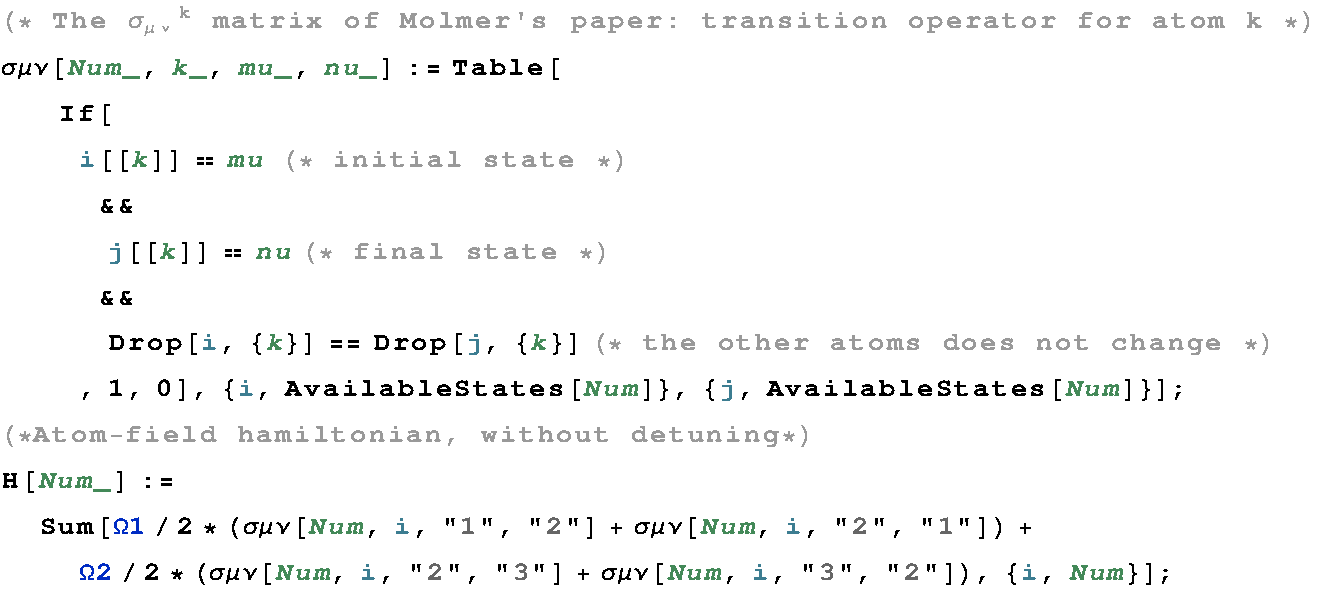
\includegraphics[width=0.8\textwidth]{MathematicaSampleCode.pdf}
  \caption{\label{Mathematica-code}\mat code to implement $\sum_j \mc{V}_{\mathrm{af}}^j$ using \emph{functionnal} programming}
\end{figure}

\begin{wrapfigure}{r}{0.45\textwidth}
  \vspace{-10pt}
  \centering
  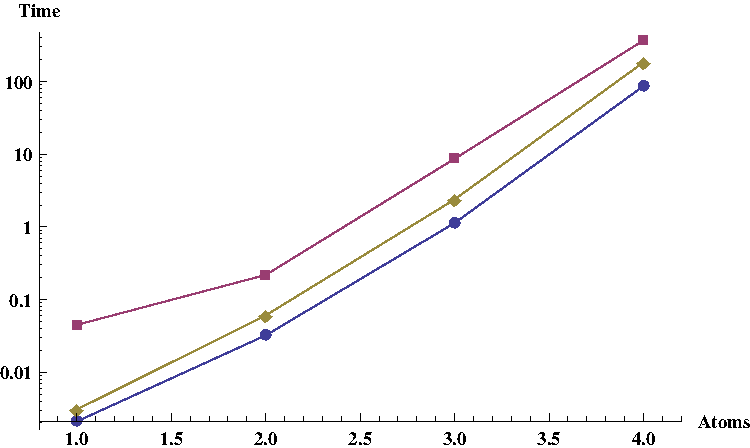
\includegraphics[width=0.45\textwidth]{benchmark.pdf}
  \caption{\label{benchmark-plot}Master equations computation time}
  \vspace{-20pt}
\end{wrapfigure}


\par This example shows an optimisation of the previous code. Such a work is not useless because the number of available states varies exponentially with the number of atoms. The \Cref{benchmark} and \Cref{benchmark-plot} give the time needed to find the master equation. This shows that my code\footnote{The reader should be aware that Calum's code does not give the same master equations as the other ones.} is the fastest, however the master equation has to be found only once. Then the interesting task is to solve it for different initial conditions and laser excitation. The master equations can be written into text files for large number of atoms. Indeed the \Cref{benchmark-plot} shows that the computation grows as the size of the density matrix, it means exponential with the number of atoms. This fast growth is linked to the states in superposition. It is hard to simulate the behaviour of quantum system using a classical computer.

\begin{table}[h]
  \centering
  \begin{tabular}{||l||c c c c||}
    \hline
    Number of atom & 1 & 2 & 3 & 4\\
    \hline \hline
    Calum's code & 3.1ms & 60.5ms & 2.39s & 3min4s\\
    Ilya's code & 44.8ms & 218ms & 8.65s & 6min8s \\
    My code & 2.1ms & 32.1ms & 1.13s & 1min27s \\
    \hline
  \end{tabular}
  \caption{\label{benchmark}Benchmark of several codes to find the master equation}
\end{table}

\section{Modelling experiments}

\par The implementation of master equation had been mainly motivated by two reasons. The first one was to try to validate a theoretical proposal of my supervisor about a means to derministically excite one single atom using a chirped laser pulse. He tried to validate his idea by numerical simulations, but at that time the decay was not implemented properly. This new implementation will then be useful to revalidate this proposal.

\par On the other hand an accurate theoretical model could be useful to predict \emph{a priori} or analyse \emph{a posteriori} the experiments. 

\subsection{STIRAP}

\begin{wrapfigure}{r}{0.5\textwidth}
  \vspace{-10pt}
  \centering
  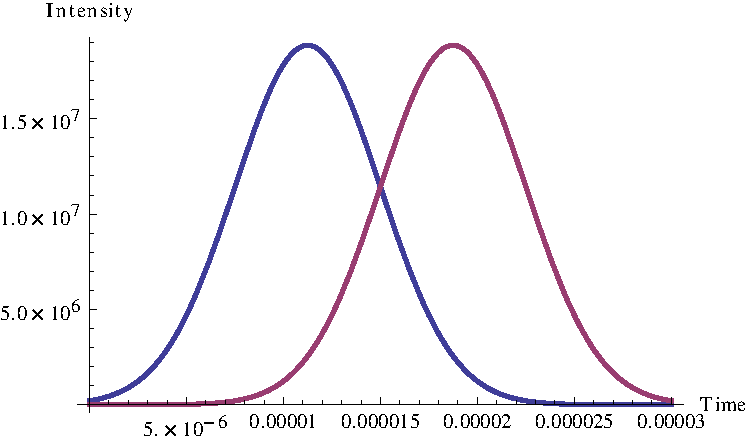
\includegraphics[width=0.5\textwidth]{STIRAP-seq.pdf}
  \caption{\label{STIRAP-seq}STIRAP laser pulse sequence\\$\Om_{ge}$ in red and $\Om_{er}$ in blue}
  \vspace{-10pt}
\end{wrapfigure}

\par The STImulated Raman Adiabatic Passage is method used to populate the Rydberg state despite the $\sqrt{N}$ dependency of the collective Rabi frequency. It consist in a two laser pulses sequence sent in a counterintuitive order. The first one $\Om_{er}$ is tunned to the transition from \ee to \rr, and the second one $\Om_{ge}$ to the transition from \ff to \ee. The \Cref{STIRAP-seq} shows the pulse sequence used to first reproduce Mølmer's results. During this sequence, a quantity defined by the following expression and called the \emph{mixing angle} $\Theta$ is swept from $0$ to $\pi/2$: \[ \tan \Theta \defi \frac{\Om_{ge}(t)}{\Om_{er}(t)} \]

\par This mixing angle could be used to express the eigenstates of the atom-field interaction hamiltonian $\mc{V}_{af}$ in the case of resonant coupling. For one atom, \cite{Berg} gives the following expressions: 

\begin{align*}
\ket{a^+} &= \sin \Th \sin \Phi \ff + \cos \Phi \ee + \cos \Th \sin \Phi \rr \\
\ket{a^0} &= \cos \Th \ff - \sin \Th \rr \\
\ket{a^-} &= \sin \Th \cos \Phi \ff - \sin \Phi \ee + \cos \Th \cos \Phi \rr
\end{align*}

\par In these expression $\Phi$ is also a function of Rabi frequencies, but it not relevant. The important information is that while the mixing angle $\Th$ runs from $0$ to $\pi/2$ allows the state \ee is never populated as it is described in the \Cref{sweeping}. The initial state is $\ff = \ket{a^0}$, and during the mixing the atom stands in state $\ket{a^0}$ because it an eigenstate of the hamiltonian.

\begin{table}[h]
  \centering
  \begin{tabular}{||c||c c||}
    \hline
    $\Th$ & $0$ & $\pi/2$\\
    \hline \hline
    $\ket{a^+}$ & $\cos \Phi \ee + \cos \Th \sin \Phi \rr$ & $\sin \Phi \ff + \cos \Phi \ee$\\
    $\ket{a^0}$ & $\ff$ & $-\rr$\\
    $\ket{a^-}$ & $- \sin \Phi \ee + \cos \Phi \rr$ & $\cos \Phi \ff - \sin \Phi \ee$\\
    \hline
  \end{tabular}
  \caption{\label{sweeping} Values taken by the eigenstates at the initial and last position \\ of the mixing angle $\Th$}
\end{table}

\par It has been shown that this sequence, based on gaussian pulses delayed by their width, has the lowest losses from non-adiabatic coupling to the $\ket{a^+}$ or $\ket{a^-}$ \cite{Berg}. This sequence can then be used in addition to the master equation to numerically simulate the STIRAP. This has been done in \cite{Molmer} and reproduced by my program\footnote{A complete version of the 

\subsection{CHIRP}
\subsection{Mark Saffman experiments}

\section{Rydberg blockade criterion}



\chapter{Automation of atom excitation}

\section{Control of the time sequence of the lasers}
\section{Microwave spectroscopy}
\section[New vacuum system and outlook]{The prospects offered by the new vacuum system}



\addchap{Conclusion}

\appendix

\chapter{Grover's algorithm\label{Grover}}

\nocite{*}
\bibliographystyle{alpha}
\bibliography{optiquequantique}

\end{document}
